\chapter{QCD primer}
\label{chap:qcd}

Quantum chromodynamics is the theory of strong interactions\footnote{A brief historical review about the development of {\sffamily QCD} may be found at \cite{historyqcd}.}. It aims to describe the interactions between elementary constituents, namely the quarks\footnote{The quarks were firstly predicted in Gell-Mann's Eightfold Way \cite{gellmann}.}, mediated by the carriers of the color force, the gluons.

The existence of color charge was proposed as an additional quantum number which would solve the violation of Pauli's exclusion principle for some particular baryons\footnote{For example, $\Delta^{++}$, which consists of three up quarks.}. Since the quarks were never experimentally evidenced, it was proposed that the strong interaction constrains the free particles to only exist in color neutral states. This particularity of {\sffamily QCD} is known as color confinement. Nevertheless, in the partonic picture\footnote{Feynman proposed that high energy nuclei are made of elementary constituents, generically called partons \cite{partons}.}, deep inelastic scattering\footnote{{\sffamily DIS} is a process during which the structure of a hadron may be probed via interaction with, in general, a lepton.} experiments between an electron and a proton confirmed the already predicted Bjorken scaling\footnote{Bjorken deduced an expression for the cross-section of the electron by imagining that it interacts electromagnetically with each parton from the proton \cite{bjorkenimf}.} of the electrons' differential cross-section.

In essence, {\sffamily QCD} is an extension of the original $\textsf{SU}(2)$ gauge theory of Yang and Mills \cite{yangmills} to local non-Abelian $\textsf{SU}(3)$ gauge transformations.

\section{Field content}
Following textbook expositions \cite{maggiore, peskin, greiner}, the {\sffamily QCD} Lagrangian $\mathcal{L}$ is constructed from symmetry principles, namely $\textsf{SO}(1,3)$ Lorentz invariance and local gauge invariance under $\textsf{SU}(3)$. The fields should transform according to irreducible representations of these groups. The quark content of the Lagrangian is described by the quark and anti-quark fields $\psi_{\alpha,i,f}(x)$ and $\overline{\psi}_{\alpha,i,f}(x)$. They are Dirac spinors (spinorial index $\alpha$), transform according to the fundamental representation of $\textsf{SU}(3)$ (color index $i=1,2,3$ or red, green, blue) and come in different flavours (flavour index $f=\overline{1,N_f}$ or up, down, strange, charm, bottom, up). The gluon fields $A_a^\mu(x)$ are Lorentz vectors and each correspond to a generator $t^a$ ($a=\overline{1,8}$) which, in the fundamental representation, is given by the Gell-Mann matrices $t^a=\lambda^a/2$.

\section{Gauge transformations} 
The quark and anti-quark fields must be invariant under local $\textsf{SU}(3)$ gauge transformations\footnote{For simplicity, all the field indices will be dropped in the following computations.}
\shadedeq{
    \psi(x)\mapsto\textsf{U}(x)\psi(x), \quad \overline{\psi}\mapsto\overline{\psi}(x)\textsf{U}^\dagger(x) 
}
with the group transformation expressible, via exponentiation, from the Lie algebra generators, with space-time dependent group parameters $\varepsilon^a(x)$, as 
\boxedeqlabel{gaugetransf}{
    \textsf{U}(x)=\exp{i\sum_a\varepsilon^a(x)t^a}
}
The gauge fields\footnote{For each algebra element $t^a$, one may introduce a gauge field $A_a^\mu$. These may be then used to construct a Lie-algebra valued gauge potential $A^\mu$. This potential depends on the chosen representation.} $A_\mu(x)=\sum\limits_a A^a_\mu(x)t^a$ must transform according to
\boxedeqlabel{gaugefields}{
    A_\mu(x)\mapsto\textsf{U}(x)A_\mu(x)\textsf{U}^\dagger(x)+\frac{i}{g}\textsf{U}(x)\big[\partial_\mu\textsf{U}^\dagger(x)\big]
}
where $g$ denotes the coupling constant. It is important to notice that one may generate gluon fields out of a null one, that is $A_\mu=0$ by applying a local gauge transformation. Such field configurations take the form
\begin{equation*}
    A_\mu^{\text{pure}}=\frac{i}{g}\textsf{U}\big(\partial_\mu\textsf{U}^\dagger\big)
\end{equation*}
and are called pure gauge fields \cite{gelisqft,eichmann}. The corresponding field strength tensor is null $F_{\mu\nu}^{\text{pure}}=0$.

One may introduce the covariant derivative\footnote{The covariant derivative has an elegant geometrical interpretation \cite{torre}: it represents the rate of change when fields from different space-time points are parallel transported along a given path. During this procedure, they are being aligned such that they may be properly compared. The corresponding connection is actually the gauge field.}
\begin{equation*}
    \textsf{D}_\mu=\partial_\mu-igA_\mu. 
\end{equation*}
Further, one may define the field strength tensor as the commutator between covariant derivatives\footnote{Since it arises as a commutator between covariant derivatives, which describe the parallel transport, the field strength tensor may be interpreted as a measure of the path dependence of parallel transport. For this reason, it is also referred to as the curvature \cite{torre}.}
\begin{equation*}
    F_{\mu\nu}=\frac{i}{g}\big[\textsf{D}_\mu,\textsf{D}_\nu\big],
\end{equation*}
which yields an expression in terms of gauge fields
\shadedeq{
    F_{\mu\nu}=\partial_\mu A_\nu-\partial_\nu A_\mu-ig\big[A_\mu,A_\nu\big]
}
or equivalently, by color components $F_{\mu\nu}=F_{\mu\nu}^at^a$, as
\begin{equation*}
    F_{\mu\nu}^a=\partial_\mu A_\nu^a-\partial_\nu A_\nu^a+gf^{abc}A_\mu^bA_\nu^c,
\end{equation*}
where $f^{abc}$ are the structure constants of the Lie algebra $\mathfrak{su}(3)$. The last term from the above equation, when plugged in the Lagrangian, will give rise to gluonic self-interactions, a particular feature of QCD. The field strength tensor gauge transforms in the usual manner as
\shadedeq{
    F_{\mu\nu}(x)\mapsto \textsf{U}(x)F_{\mu\nu}(x)\textsf{U}^\dagger(x)
}

\section{QCD Lagrangian} 
One may now proceed to constructing the Lagrangian. The quark content is that of a free fermionic Lagrangian\footnote{After replacing the partial derivative with the covariant derivative, the Lagrangian will also contain an interaction term
\begin{equation*}
    \mathcal{L}_{\textsf{int}}=g \overline{\psi} \gamma^\mu A_\mu^a t^a \psi.
\end{equation*}}, but built with covariant derivatives, in order to satisfy gauge invariance
\begin{equation*}
    \mathcal{L}_{\textsf{quarks}}=\overline{\psi}(x)\big(i\slashed{\textsf{D}}-\textsf{M}\big)\psi(x),
\end{equation*}
where $\textsf{M}=\textsf{Diag}\left\{m_1,\ldots,m_{N_f}\right\}$ is the diagonal quark mass matrix in flavour space\footnote{In the Standard Model, the quark mass matrix is no longer diagonal. After spontaneous symmetry breaking, the mixing between different flavoured quark masses is given by the {\sffamily CKM} matrix \cite{pdg}.}. 

The dynamics of the gluon fields is described by the following construction\footnote{It is important to notice that such a construction contains not only standard kinetic terms but also interaction vertices with three gluons, which are proportional to $g$ and four gluons, proportional to $g^2$.}
\begin{equation*}
    \mathcal{L}_{\textsf{gluons}}=-\frac{1}{2}\textsf{Tr}\left\{F_{\mu\nu}F^{\mu\nu}\right\},
\end{equation*}
where the color tracing over the contraction of field strength tensors assured gauge invariance. Equivalently, one may rewrite the above expression in terms of color components as
\begin{equation*}
    \mathcal{L}_{\textsf{gluons}}=-\frac{1}{4}F_{\mu\nu}^aF^{a,\mu\nu},
\end{equation*}
valid in the fundamental representation, where $\textsf{Tr}\left\{t^at^b\right\}=\delta^{ab}/2$. Therefore, the {\sffamily QCD} Lagrangian takes the form
\boxedeqlabel{qcd6}{
    \mathcal{L}_{\textsf{QCD}}=\overline{\psi}(x)\big(i\slashed{\textsf{D}}-\textsf{M}\big)\psi(x)-\frac{1}{4}F_{\mu\nu}^aF^{a,\mu\nu}
}

The corresponding Yang-Mills action expressed in flat coordinates is given by
\begin{align}\label{yangmills}
    \textsf{S}=\int\mathrm{d}^4x\left(-\frac{1}{2}\textsf{Tr}\left\{F_{\mu\nu}F^{\mu\nu}\right\}\right),
\end{align}

\section{Field equations} 
The variational derivatives with respect to the color spinor fields give the colored Dirac equations
\begin{equation*}
    (i\slashed{\textsf{D}}-\textsf{M})\psi=0,    
\end{equation*}
and similarly for the anti-quark fields
\begin{equation*}
    \overline{\psi}(i\overleftarrow{\slashed{\textsf{D}}}-\textsf{M})=0.    
\end{equation*}
The Euler-Lagrange equations corresponding to the gluon fields yield the Yang-Mills equations, or equivalently, colored Maxwell equations\footnote{There is an additional equation, called the Bianchi identity, which follows from the definition and properties of $F_{\mu\nu}$. It may be expressed as \cite{tong}
\begin{equation*}
    \textsf{D}_\mu^{\phantom{*}*}F^{\mu\nu}=0,
\end{equation*}
where we introduced the dual field strength tensor as
\begin{equation*}
    ^*F^{\mu\nu}=\frac{1}{2}\epsilon^{\mu\nu\rho\sigma}F_{\rho\sigma}.
\end{equation*}}
\shadedeq{
    \textsf{D}_\nu F^{\nu\mu}=gJ^\mu
}
in which $J^\mu=\sum\limits_a J^{a,\mu} t^a$ with $J^{a,\mu}=\overline{\psi}\gamma^\nu t^a\psi$ being the color current. The color current is covariantly conserved $\textsf{D}_\mu J^\mu=0$.

%This is an example chapter. 
%\section{Math and formulae}
%For inline math use \(t_hi^s\) or $t_{hi}s$ ---the recommended option is the first one---.
%Inline math should be used for short expressions
%or when referring to functions, \(f(x)\) or variable names like $x$.
%
%For unnumberd equations use
%\[
%\mathcal{S} = \int_{t_0}^{t_1} \mathcal{L} \dd{t}
%\]
%
%and
%
%\begin{equation*}
%\var \mathcal{S} = 0.
%\end{equation*}
%
%For numbered equations use
%\begin{equation}
%\label{eq:time-evolution-heisenberg}
%i \hbar \dv{A_H(t)}{t} = \comm{A_H(t)}{H}.
%\end{equation}
%
%\subsection{Details}
%
%If you use a label for something, like an equation, you can reffer to it later in text, see eq.~\cref{eq:time-evolution-heisenberg}.
%For more details regarding the Heisenberg picture of Quantum Mechanics, see~\cite{Dirac1967, Sakurai2011} and also the
%lecture notes~\cite{Baran, Zus}. Equation~\cref{eq:time-evolution-heisenberg} reminds us of Hamilton's equations
%\begin{align*}
%  \dot{q}_k = [q_k,H], && \dot{p}_k = [p_k,H].
%\end{align*}
%
%An other important picture of Quantum Mechanics is the Schrödinger one. In this formulation the observables are time
%independent and the states are evolving in time. The time evolution is given by the well-known Schrödinger equation
%\boxedeq{
%  i \hbar \pdv{t} \ket{\Psi} = H \ket{\Psi}.
%}
%
%If you have a very long formula, you can split it like this
%\begin{equation}
%\label{eq:long}
%\begin{split}
%\left(1+x\right)^n  &=  1 + nx + \frac{n\left(n-1\right)}{2!}x^2 \\
% &+ \frac{n\left(n-1\right)\left(n-2\right)}{3!}x^3 \\
% &+ \frac{n\left(n-1\right)\left(n-2\right)\left(n-3\right)}{4!}x^4 \\
% &+ \ldots
%\end{split}
%\end{equation}
%
%\subsubsection{Definitions and theorems}
%
%\begin{definition*}[Joint probability]
%Given two events $A$ and $B$, their joint probability, \(P(A \cap B)\), is the probability of the two events to occur simultaneously.
%\end{definition*}
%
%\begin{theorem}[Pythagorean theorem]
%    	This is a theorem about right triangles and can be summarised in the next equation 
%    	\shadedeq{
%			x^2 + y^2 = z^2    	
%    	}
%
%\end{theorem}
%
%\begin{remark}
%	Some remark, blablabla.
%\end{remark}
%
%\begin{proof}
%Some proof, done!
%\end{proof}
%
%\section{Tables}
%
%\begin{table}[ht]
%\centering
%\caption{Angular momentum}
%\label{tab:my-label}
%\begin{tabular}{llll}
%\toprule
%Type & Commutation relations & Eigenvalues & \\
%\midrule
%General & \(\comm{J_i}{J_j} = i \hbar \varepsilon_{ijk} J_k\)  & \(\vec{J}^2 \ket{jm} = j(j+1) \hbar^2 \ket{jm}\) & \(J_z \ket{jm} = m \hbar \ket{jm}\) \\ 
%Orbital  & \(\comm{L_i}{L_j} = i \hbar \varepsilon_{ijk} L_k\)  & \(\vec{L}^2 \ket{lm} = l(l+1) \hbar^2 \ket{lm}\) & \(L_z \ket{lm} = m \hbar \ket{lm}\) \\
%Spin  & \(\comm{S_i}{S_j} = i \hbar \varepsilon_{ijk} S_k\)  & \(\vec{S}^2 \ket{sm} = s(s+1) \hbar^2 \ket{sm}\) & \(S_z \ket{sm} = m \hbar \ket{sm}\) \\
%\bottomrule
%\end{tabular}
%\end{table}
%
%\section{Figures}
%
%Figure~\cref{fig:parabolic} shows a simple figure. Two figures side by side in fig.~\cref{fig:hyperbolic}.
%
%\begin{figure}[H]
%  \centering
%  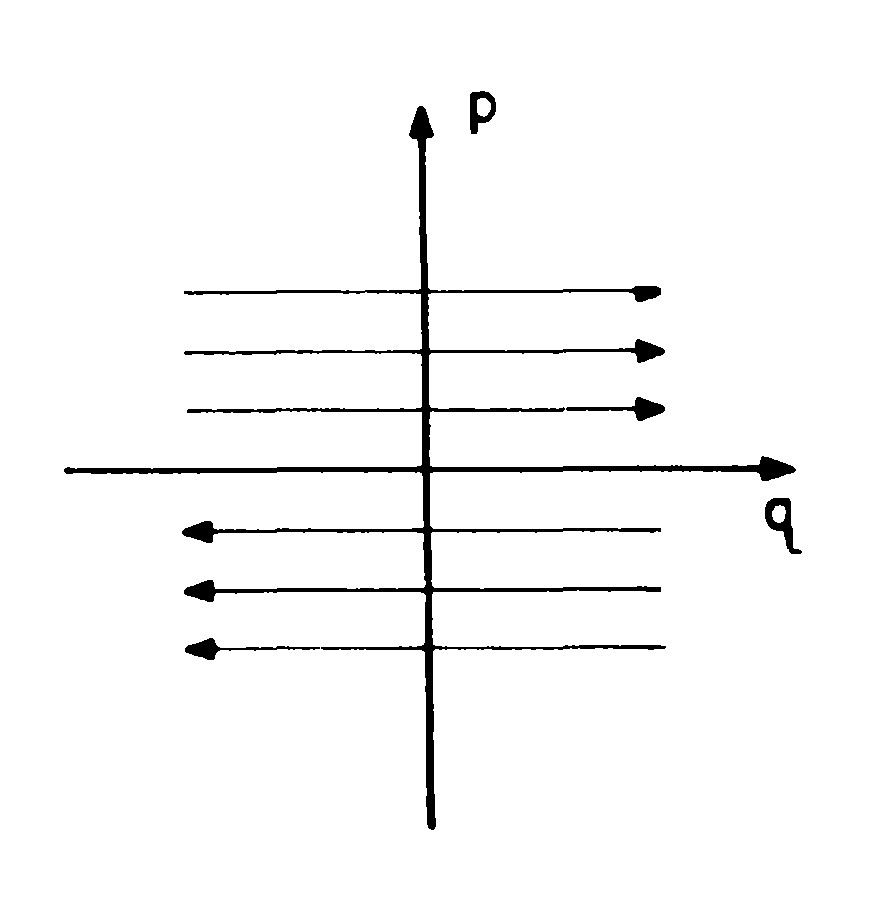
\includegraphics{parabolic}
%  \caption{Parabolic fixed point}
%\label{fig:parabolic}
%\end{figure}
%
%\begin{figure}[ht]
%  \centering
%  \begin{subfigure}[t]{0.45\textwidth}
%    \centering
%    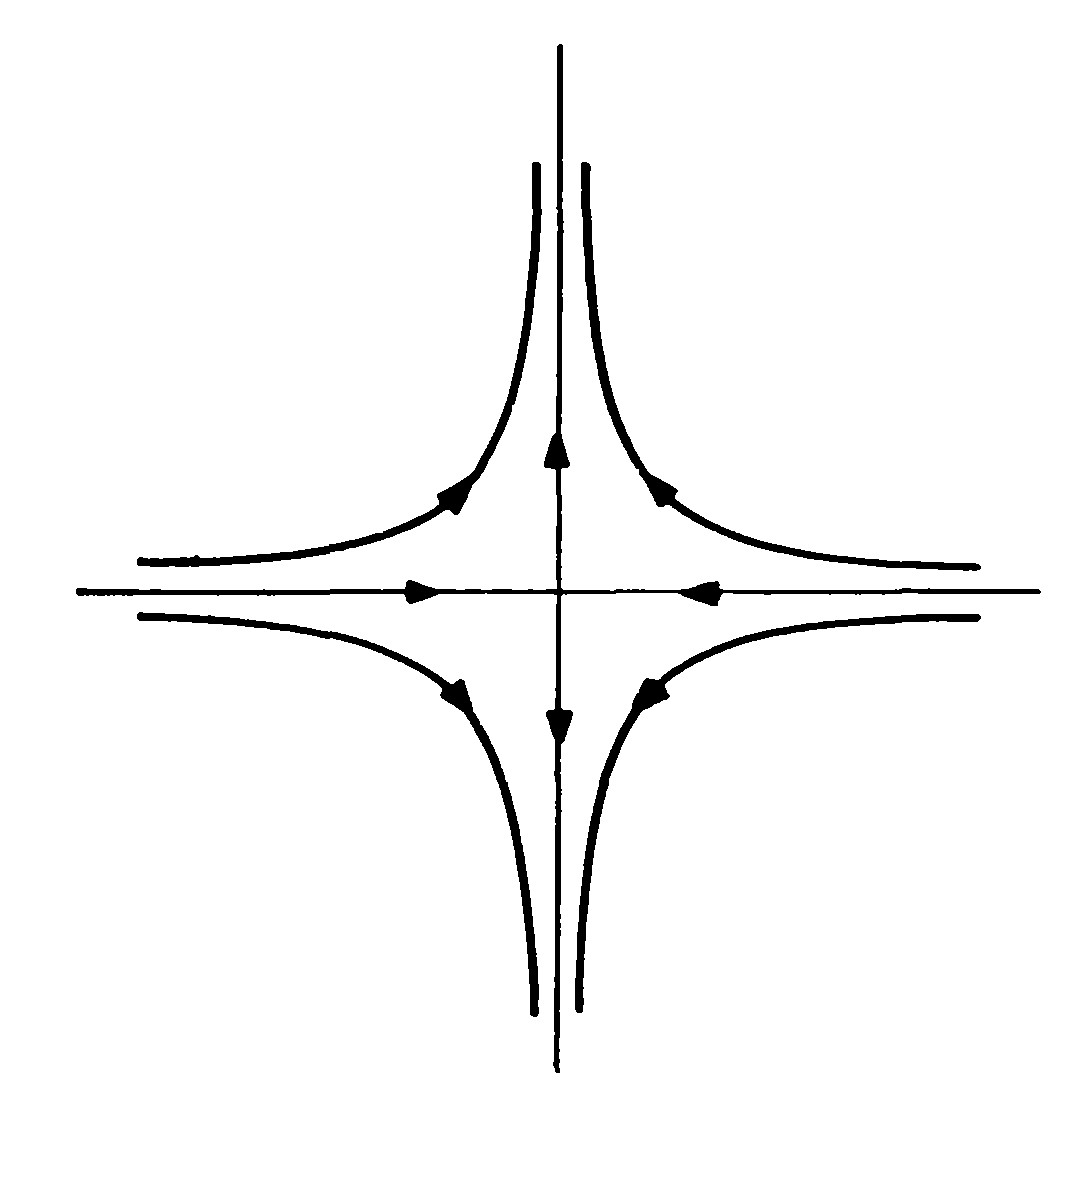
\includegraphics{hyperbolic}
%    \caption{Hyperbolic fixed point}
%  \end{subfigure}
%~
%  \begin{subfigure}[t]{0.45\textwidth}
%    \centering
%    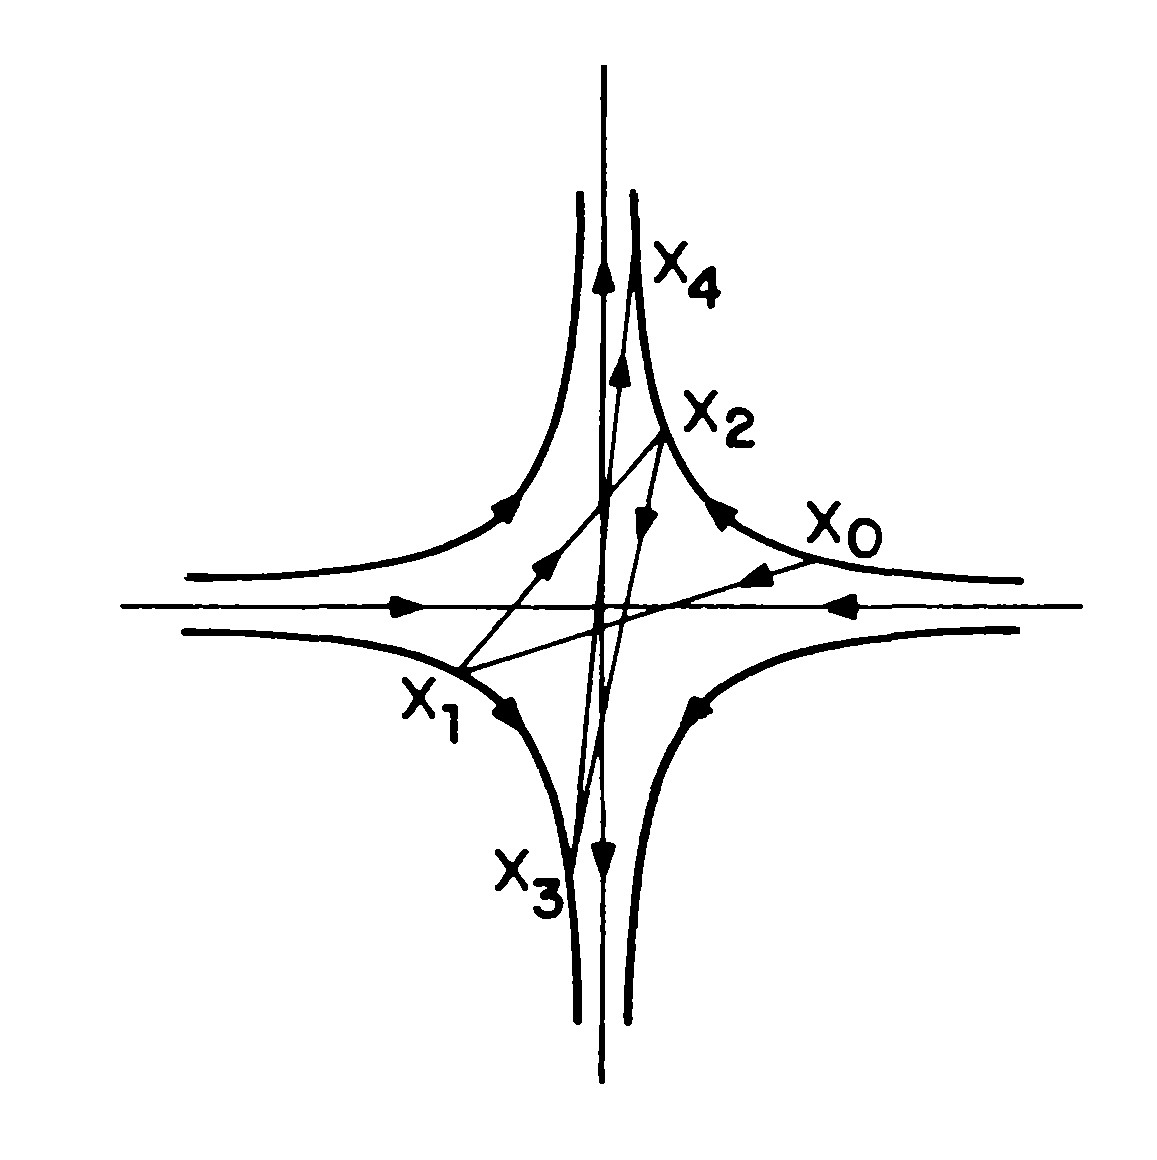
\includegraphics{hyperbolic-reflection}
%    \caption{Hyperbolic-with-reflection fixed point}
%  \end{subfigure}
%\caption{}
%\label{fig:hyperbolic}
%\end{figure}